\section{Data Visualization and Insights}\label{sec:data_visualization}

Now that our probe data and SST tools are integrated, we can use various visualization tools to analyze our data and gain valuable insights. For example, if we want to identify which type of requests are most common in our microservices, we can leverage the data stored in Neo4j (our SST tool) and connect it to a visualization platform.

To demonstrate this, we will use Tableau as our visualizer tool. By linking Tableau with Neo4j, we can create interactive charts and dashboards to better understand request patterns, trends, and system behavior. This approach will help us make informed decisions based on clear and structured data representation.

\begin{figure}[H]
    \centering
    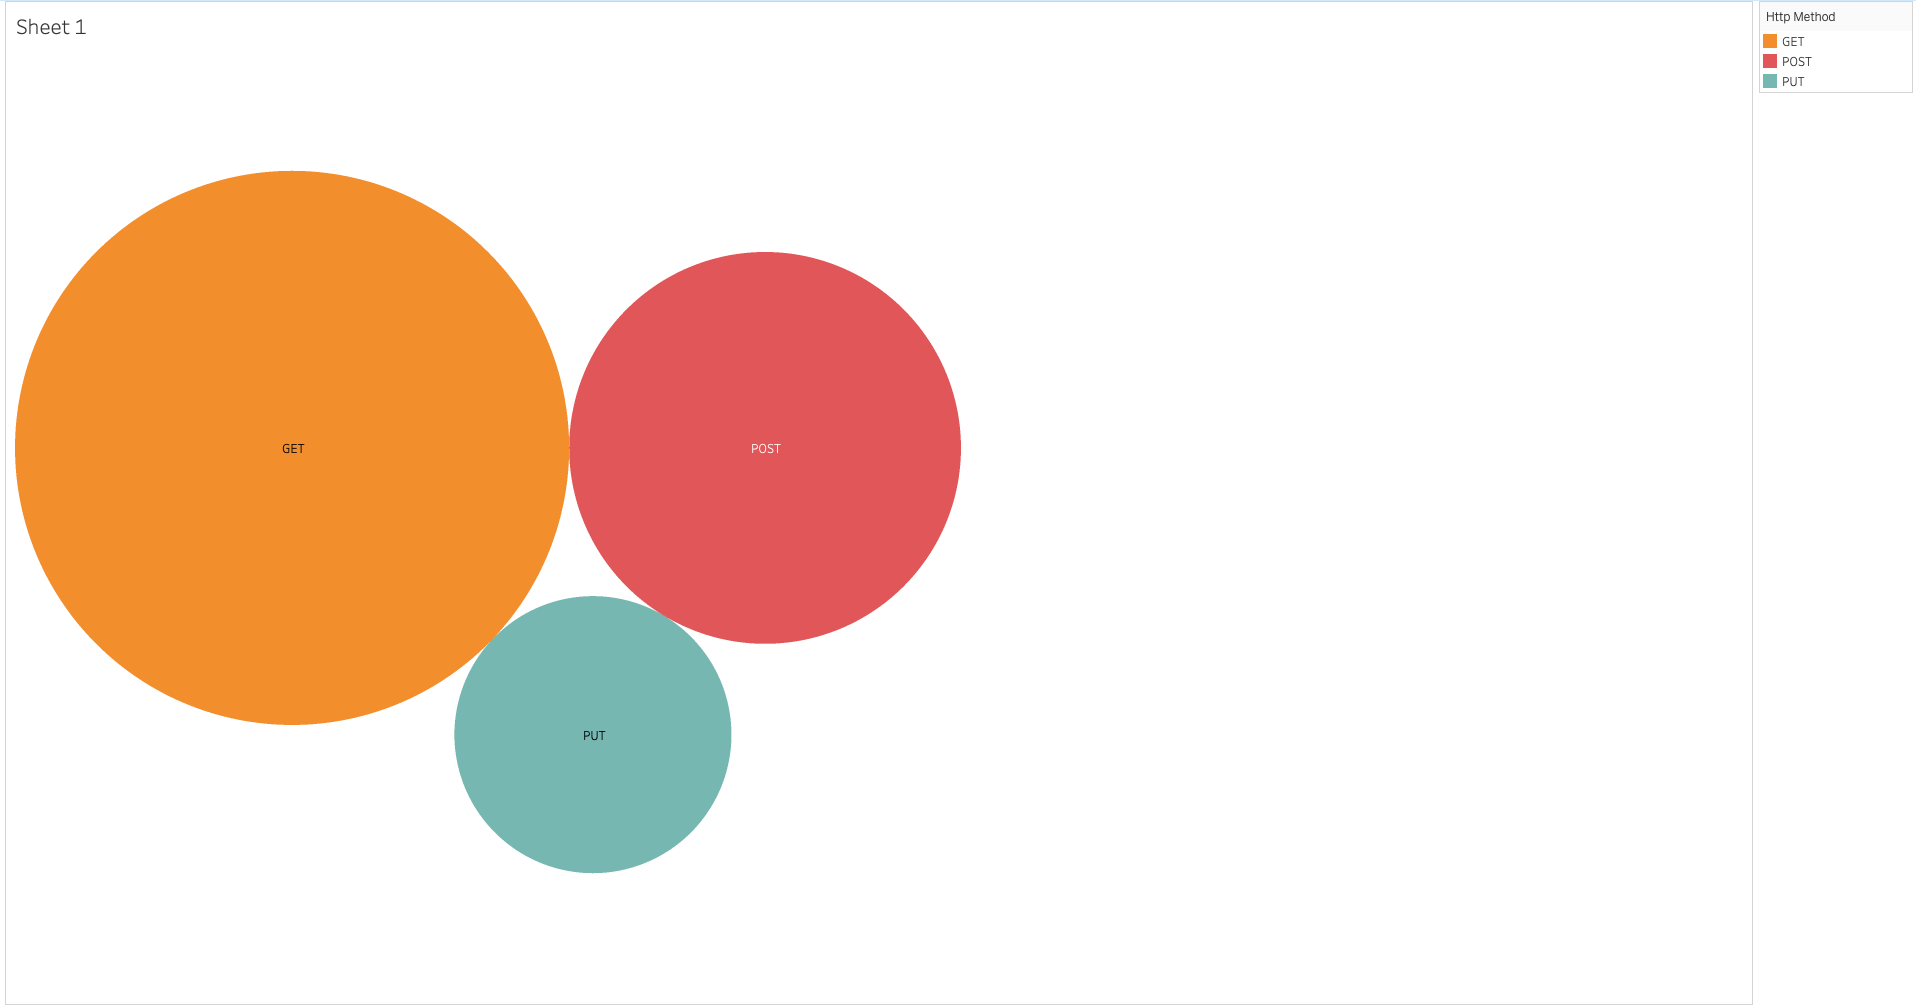
\includegraphics[width=1\textwidth]{figures/tableau_1.png}
    \caption{REST API requests dominance}
    \label{fig:tableau}
\end{figure}